% !TeX spellcheck = <Dutch>

\chapter{Praktische uitwerking}
\vspace{-3cm}
Het annoteren van afbeeldingen is \'{e}\'{e}n van de onderdelen binnen de \textit{Profile Manager} van CX Social. De \textit{Profile Manager} is een nieuwe feature die gebruikers moet helpen bij het beheren van hun sociale media profielen. Een thema kan aangemaakt worden voor Facebook of Twitter dat een omslag-en/of profielfoto bevat. Eens een omslagfoto ge\"{u}pload is, is het mogelijk om annotaties toe te voegen. Dit kan simpelweg tekst zijn maar ook KPI's kunnen op de afbeelding geplaatst worden. Gebruikers kunnen voor geconnecteerde profielen instellen welk thema op welk tijdstip actief moet zijn. De aangemaakte afbeeldingen worden dan op de ingestelde tijdstippen ge\"{u}pload naar het juiste profiel. 


\section{Frontend implementatie}
Een groot deel van de frontend code van CX Social is geschreven met React. Met React kunnen makkelijk componenten aangemaakt worden om zo complexe interfaces aan te maken. Om de \textit{Profile Manager} zo modulair mogelijk te maken worden de verschillende \textit{features} opgesplitst in React componenten. 

\subsection{Aanmaken van een thema} \label{AanmakenVanEenThema}

 %2o zijn er heel wat componenten beschikbaar waarmee gemakkelijk functionaliteit aan een pagina kan toegevoegd worden.
Om een thema aan te maken zijn een naam, een \textit{service} %CHECK IF ITS ITALIC EVERYWHERE!!! 
en twee velden nodig om afbeeldingen te uploaden (zie Figuur \ref{fig:ThemeComponent}). Aangezien dezelfde functionaliteit vereist is bij het aanmaken en editeren van een thema, wordt gebruik gemaakt van een React component. De \texttt{ThemeComponent} stelt een volledig thema voor en zal alle veranderingen hieraan afhandelen. Dit betekent dus zowel het ingeven van de naam en service als het bijhouden van de geannoteerde afbeeldingen. Uiteindelijk is het deze component die instaat voor alle interacties met een thema. 
%Zowel het aanmaken als editeren van een thema verwachten dezelfde functionaliteit.
%Eens een thema aangemaakt is, kan het later ook aangepast worden. Omdat dezelfde functionaliteit op twee verschillende pagina's nodig is, wordt hiervoor een React component aangemaakt: de \texttt{Theme} component (zie Figuur \ref{fig:ThemeComponent}). 
Bij het aanmaken van de \texttt{ThemeComponent} dienen enkele eigenschappen meegegeven te worden. Eerst en vooral wordt het, uit de databank opgehaalde, thema meegegeven indien dit beschikbaar is. %ADD SOME INFO OVER HOW IT IS IN VIEW, WHEN NO THEME IS SELECTED!

Het account \textit{Identity Document} (ID), \textit{Cross-site requrest forgery} (CSRF) token, beschikbare services, en de annotatiepermissie zijn verplichte eigenschappen van de component. Deze eigenschappen zullen nooit veranderen tijdens de levensduur van de component, het zijn dus constanten. Het CSRF token wordt aan het formulier toegevoegd om ongeauthoriseerde acties in applicaties te voorkomen. Met het gegenereerde token wordt ervoor gezorgd dat geen ongeldige \textit{requests} gemaakt kunnen worden naar de pagina. Dit maakt het dus onmogelijk om thema's aan te maken zonder vanop een kwaadaardige sites.  %http://stackoverflow.com/questions/5207160/what-is-a-csrf-token-what-is-its-importance-and-how-does-it-work
Niet elke gebruiker heeft dezelfde rechten in CX Social. Binnen een bepaald plan zijn verschillende gebruikersrollen beschikbaar. Zo zijn er gewone gebruikers, \textit{admins}, managers, \textit{editors}, \textit{contributors} en \textit{analytics users}, elk met hun eigen rechten. Permissies, die aan de gebruiker werden toegekend, worden meegegeven aan de Theme component om de annoteer \textit{feature} al dan niet beschikbaar te stellen. Ieder inputveld bevat een \texttt{onChange} event waarmee veranderingen afgehandeld kunnen worden. 

\begin{figure}[H]
	\centering
	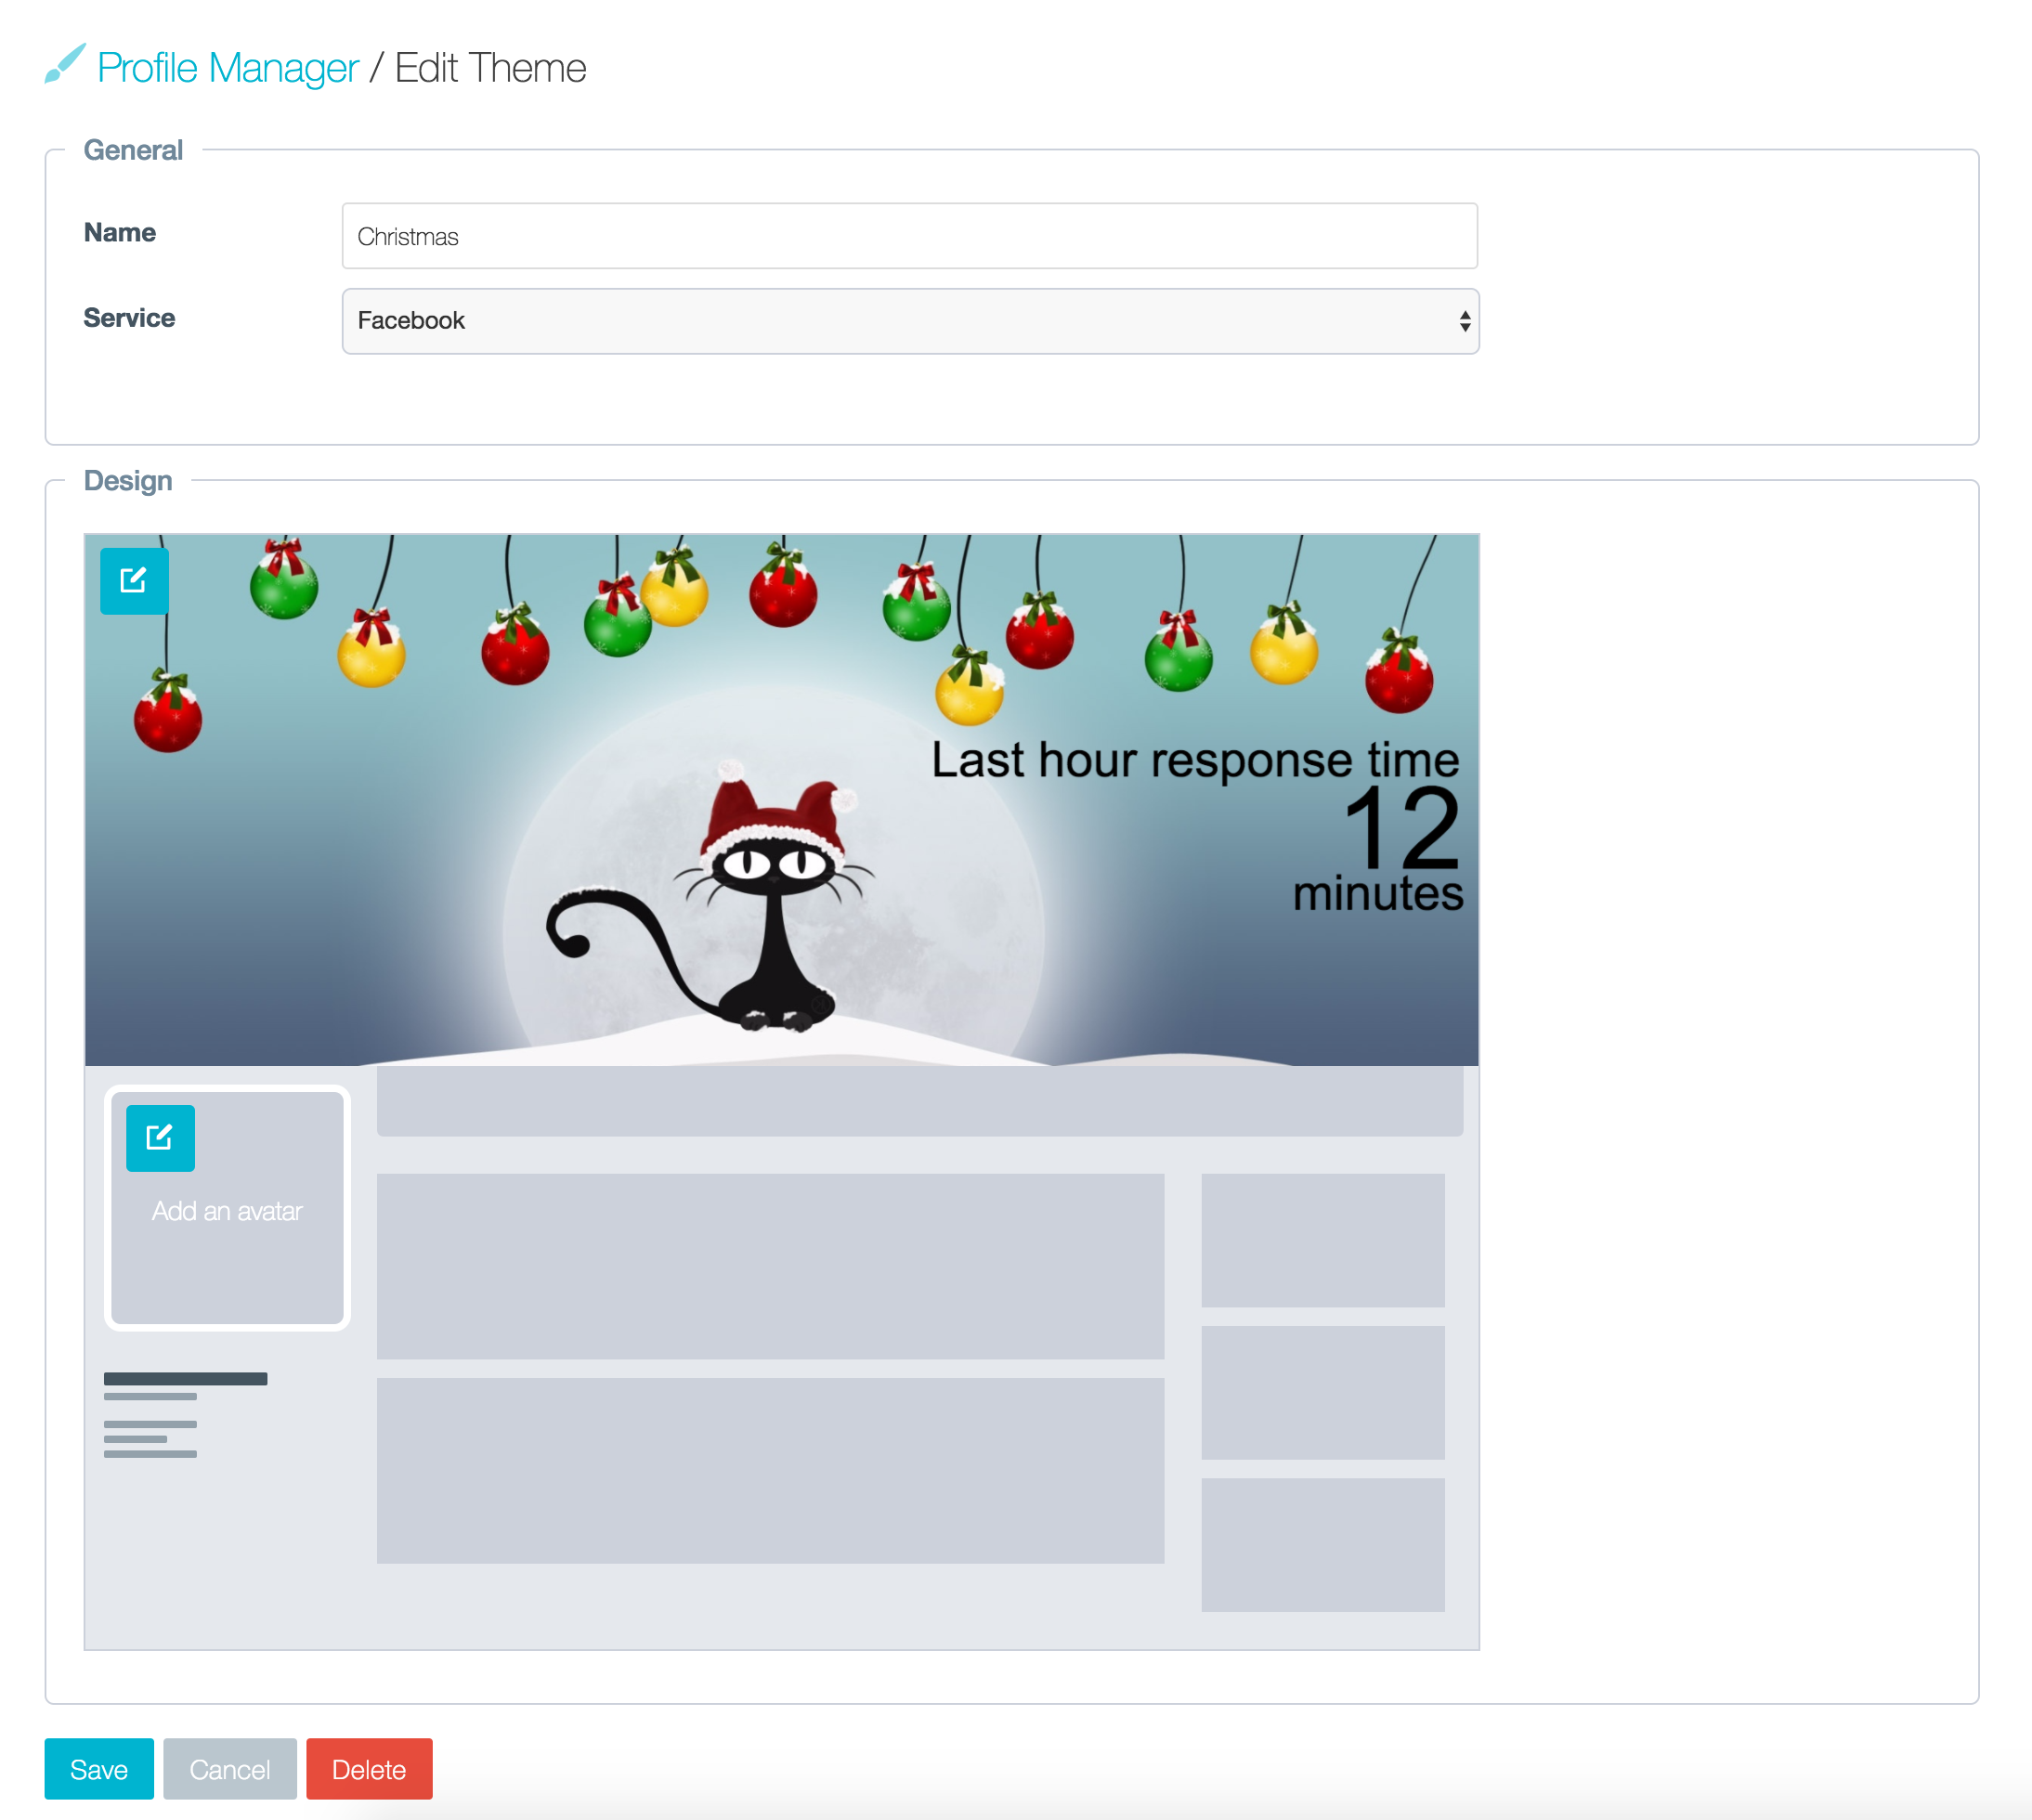
\includegraphics[width=0.6\textwidth]{Figuren/ThemeComponent.png}
	\caption{ThemeComponent in de editeer pagina}
	\label{fig:ThemeComponent}
\end{figure} 



Zoals te zien in codevoorbeeld \ref{lst:ThemeComponentDropdown} wordt de state van de component ge\"{u}pdatet wanneer een verandering aan de inputvelden plaatsvindt. De state van de component kan, in tegenstelling tot de eigenschappen (props), wel veranderen binnen het component. De state kan aangepast worden met behulp van  de \texttt{setState()} methode. 

\begin{lstlisting}[caption={Theme component - Dropdown},label=lst:ThemeComponentDropdown,language=javascript]
<select className={this.state.saving && this.state.service === '' ? 'error 		fieldset-input' : 'fieldset-input'} id="service" name="service" ref="service" value={this.getService()}
	onChange={function (event) {
		this.setState({service: event.target.value});
	}.bind(this)}>
	{this.props.services.map(function (service) {
		return <option key={service} value={service}>{this.capitalize(service)}</option>
	}.bind(this))}
</select>
\end{lstlisting}

Naast het ingeven van een naam en \textit{service} voor het thema, kunnen ook een omslag-en profielfoto toegevoegd worden. Het uploaden van de afbeeldingen wordt afgehandeld door een reeds bestaande component. Deze zal een, door de gebruiker geselecteerde, foto uploaden naar de \textit{fileserver} en op de pagina weergeven. Eens een afbeelding aanwezig is, is het mogelijk om annotaties toe te voegen. Om een afbeelding te annoteren wordt een pop-upvenster geopend. Aangezien dit venster een volledig nieuwe \textit{template} is, dienen enkele eigenschappen van het thema meegegeven te worden. Als parameters in de URL worden zowel de \textit{service} als de bestandsnaam van de afbeelding op de fileserver meegegeven. Beide parameters zijn nodig om het canvas op te stellen. De \textit{service} bepaald immers de dimensies van het canvas aangezien deze verschillen voor zowel Facebook als Twitter. Via de bestandsnaam kan de correcte afbeelding ingeladen worden in het pop-upvenster.

Zoals reeds besproken in sectie \ref{vergelijkingBibliotheken}, lijkt Fabric.js de beste keuze te zijn om dit project uit te werken. Aangezien niet alle functionaliteit van deze bibliotheek van toepassing zijn op dit project, wordt een \textit{custom build} aangemaakt. Deze bevat de tekst, interactieve tekst, animatie, serialisatie, interactie en node \textit{features}. Bij het openen van het pop-upvenster wordt het \texttt{ThemeAnnotations} component ge\"{i}nitialiseerd met de nodige eigenschappen. Deze zijn het account ID, de bestandsnaam van de afbeelding, de \textit{service} en een kleurenpallet. Tussen deze kleuren en eender welke hexadecimale waarde kan gekozen worden tijdens het stylen van de annotaties.

\begin{lstlisting}[caption={ThemeAnnotations component - initialisatie}\label{ThemeComponentDropdown},language=javascript]
$(document).ready(function() {
	var annotationProps = {
		accountId: '{{account.id}}',
		image: '{{image}}',
		service: '{{service}}',
		colors:  [
		"#FF691F",
		"#FAB81E",
		"#7FDBB6",
		"#19CF86"
		]};
		
	ReactRenderer.render(
		React.createElement(ThemeAnnotations, annotationProps),
		document.getElementById('annotations'),
		$.noop()
	);
});
\end{lstlisting}

\subsection{Annoteren van de afbeelding}\label{AnnoterenVanAfbeelding}
Het annoteren van een ge\"{u}ploade afbeelding vindt plaats in een  pop-upvenster. Zoals vermeld in sectie \ref{AanmakenVanEenThema}, wordt ook hier een React component voor aangemaakt. Deze component handelt elke verandering aan het canvas en zijn objecten af en staat ook in voor het exporteren van het volledige canvas. 

Wanneer het canvas element aanwezig is in het DOM, wordt het canvas ge\"{i}nitialiseerd. Dit gebeurt in de \texttt{componentDidMount()} functie van de React component. Zowel Facebook als Twitter verwachten omslagfoto's van een bepaalde resolutie. Wordt hier niet aan voldaan, zullen de foto's worden geschaald. Om kwaliteitsverlies te voorkomen, worden de foto's dus best met de correcte resolutie g\"{u}pload. Helaas kan het canvas niet aangemaakt worden met de verwachte dimensies van de foto's. Bij Facebook zou dit een canvas van 828 op 315 pixels zijn terwijl dit voor Twitter een canvas van 1500 op 500 pixels zou zijn. Het is helemaal niet handig voor een gebruiker om op een canvas met een breedte van 1500 pixels te werken. Daarom worden de dimensies van het canvas dynamisch berekend. Dankzij de berekeningen kan ook de ratio (hoogte ten opzichte van breedte) van de afbeeldingen behouden worden. Wanneer de afbeelding dan uiteindelijk gegenereerd wordt, moeten de dimensies simpelweg met dezelfde verkleiningsfactor vermenigvuldigd worden om zo een afbeelding met gewenste dimensies te bereiken. Het canvas wordt als volgt aangemaakt:

\begin{lstlisting}[language=javascript]
getInitialState: function () {
	return {
		facebookCover: {width: '828', height: '315'},
		twitterCover: {width: '1500', height: '500'}
	}
},
componentDidMount: function () {
	var dimensions = {};
	if (this.props.service === 'twitter') {
		ratio = this.state.twitterCover.width / this.state.twitterCover.height;
		dimensions = this.state.twitterCover;
	}
	else if (this.props.service === 'facebook') {
		ratio = this.state.facebookCover.width / this.state.facebookCover.height;
		dimensions = this.state.facebookCover;
	}
		
	this.canvas = new fabric.Canvas('annotationCanvas', {
		width: this.refs.container.offsetWidth,
		height: this.refs.container.offsetWidth / ratio,
		preserveObjectStacking: true,
		renderOnAddRemove: true,
		multiply: ratio,
		service: this.props.service,
		dimensions: dimensions,
	});
}
\end{lstlisting}

Eens het canvas bestaat, kunnen objecten toegevoegd worden. Met behulp van de \texttt{fromUrl(url, callback)} methode van het \textit{Image} object kan een afbeelding aan het canvas toegevoegd worden. De URL wordt simpelweg opgesteld aan de hand van de meegegeven bestandsnaam. Eens de afbeelding ingeladen is worden enkele transformaties uitgevoerd om de afbeelding gepast weer te geven. Zo wordt de afbeelding gecentreerd, geschaald tot de volledige breedte van het canvas en naar de achtergrond van het canvas verplaatst. Deze transformaties zorgen ervoor dat het volledige canvas bedekt wordt door de afbeelding en dat alle andere objecten, zoals tekst en KPI's, bovenop de afbeelding terecht zullen komen. 

%ZIE BIJLAGE HANDLEANNOTATIONS FUNCTION VANAF REGEL ..... (gwn inladen van afbeelding)

Gewone tekst wordt als een \texttt{IText} object toegevoegd aan het canvas. Hierdoor is de gebruiker in staat om de tekst aan te passen in het canvas zelf en hoeft dus geen extra inputveld te worden voorzien. Net zoals de afbeelding naar de achtergrond wordt gestuurd, worden tekst objecten naar de voorgrond gebracht met behulp van de \texttt{bringToFront()} functie van het canvas. Een tekst object wordt als volgt aan het canvas toegevoegd:

\begin{lstlisting}[language=javascript]
var text = new fabric.IText('click here to add your text', {
	fontFamily: 'Arial',
	left: this.canvas.width / 2,
	top: this.canvas.height / 2,
	fontSize: 30,
	transparentCorners: false,
	textAlign: 'left',
	lockUniScaling: true,
	borderColor: '#00b4d0',
	cornerColor: '#00b4d0',
	centeredScaling: true,
	textType: 'text',
});

this.canvas.add(text);
this.canvas.bringToFront(text);
\end{lstlisting}

Naast de standaard eigenschappen zoals tekstgrootte, lettertype en positie op het canvas bevat het object een extra \texttt{textType} eigenschap. Deze maakt duidelijk dat het om gewoon tekst object gaat en niet over een KPI. Na het toevoegen van het object aan het canvas wordt het naar de voorgrond gebracht om er zeker van te zijn dat de tekst bovenop de afbeelding terecht komt. 

De gebruiker kan kiezen tussen vier verschillende soorten KPI's: 'respons tijdens het laatste uur', 'respons tijdens de laatste dag', 'geholpen gebruikers de laatste dag' en 'geholpen gebruikers de laatste zeven dagen'. Bij het toevoegen van een KPI aan het canvas moet het soort KPI dus ook opgeslagen worden.% Ook dient een waarde toegekend te worden zodat de gebruiker een idee heeft van de uiteindelijke afbeelding. 
Wat een probleem vormt tijdens de uitwerking is de positionering van de KPI's. Aangezien dit variabele getallen zijn, is een getal van vier of vijf cijfers lang niet uit te sluiten. Hoewel de inhoud van een \texttt{IText} object uit te lijnen is (links, rechts of gecenteerd), is dit pas merkbaar bij tekst bestaande uit meerdere lijnen. Daarom wordt geopteerd voor een \texttt{Textbox} object om de KPI's weer te geven. Tijdens het initialiseren van dit object kan de breedte ingesteld worden waardoor ook een enkel woord uitgelijnd kan worden. Via een \textit{switch} statement wordt de correcte type KPI aan het object toegekend (zie onderstaand codefragment). 

\begin{lstlisting}[language=javascript]
var mockValue = '';
switch (value) {
	case 'last_hour_response_time':
		mockValue = '12';
		break;
	case 'last_day_response_time':
		mockValue = '30';
		break;
	case 'seven_days_serviced_users':
		mockValue = '218';
		break;
	case 'last_day_serviced_users':
		mockValue = '72';
		break;
	default:
		mockValue = 'NaN'
}

var KPI = new fabric.Textbox(mockValue, {
	fontFamily: 'Arial',
	left: this.canvas.width / 2,
	top: this.canvas.height / 2,
	fontSize: 70,
	textAlign: 'center',
	textType: 'kpi',
	kpiType: value,
	width: 400,
	editable: false
});

this.canvas.add(KPI);
this.canvas.bringToFront(KPI);
\end{lstlisting}

%ADD CoDE FRAGMENT TO DIS OR JUST DELETE?
Gebruikers kunnen ook gebruik maken van een \textit{template}. Dit zal enkele tekst objecten op het canvas plaatsen alsook de gekozen KPI. Zo kunnen gebruikers zeer eenvoudig hun afbeeldingen annoteren met bijvoorbeeld: 'We took care of 500 customers last week'. Alle elementen worden gecentreerd op het canvas en kunnen door de gebruiker zelf nog aangepast worden. 

\subsection{Editeren van tekst}
E\'{e}n van de \textit{features} tijdens het annoteren van een afbeelding is het stylen van de tekst. Dit maakt het mogelijk eigenschappen zoals tekstgrootte, lettertype, kleur en gewicht (vet of schuin) aan te passen. Om dit op een modulaire manier te verwezenlijken, wordt gebruik gemaakt van een React component. Aan de \texttt{TextEditor} component worden enkele eigenschappen meegegeven om een bestaand tekst object aan te kunnen passen. Onder deze eigenschappen valt een \texttt{onChange()} functie, een \texttt{currentSettings} object en een \texttt{selectedColor} string. Wanneer een object in het canvas wordt geselecteerd, wordt het  \texttt{object:selected} event getriggered. In de \textit{handler} van dit event wordt, na confirmatie dat het om een tekst object gaat, de state van de \texttt{Theme} component aangepast naar de huidige instellingen van het object: 

\begin{lstlisting}[language=javascript]
this.canvas.on({'object:selected': function () {
	var object = null;
	if (this.isTextSelected()) {
		object = this.canvas.getActiveObject();

		this.setState({
			currentSettings: {
				fontSize: object.getFontSize(),
				fontWeight: object.getFontWeight(),
				fontFamily: object.getFontFamily(),
				fontStyle: object.getFontStyle(),
				fontColor: object.getFill(),
				textAlign: object.getTextAlign(),
			}, textSelected: true, objectInfo: kpiType
		});
	}}.bind(this)
});
\end{lstlisting}

De update van de state zal ervoor zorgen dat de component opnieuw gerendered wordt. Met behulp van een check in de \texttt{render} functie van de \texttt{Theme} component kan de \texttt{TextEditor} component ge\"{i}nitialiseerd worden met de nodige eigenschappen (zie codefragment \ref{lst:ThemeComponentTextEditor}). De belangrijkste eigenschap is de \texttt{onChange()} functie die vanuit de \texttt{TextEditor} component getriggered kan worden. Het triggeren gebeurt wanneer een inputveld van de editor verandert. De huidige instellingen worden opgehaald en de nodige aanpassingen worden gemaakt. Uiteindelijk wordt de state aangepast en wordt de \texttt{onChange()} functie aageroepen met de nieuwe instellingen als parameter (zie codefragment \ref{lst:TextEditorComponentBold}). Bij het triggeren van de \texttt{onChange()} zal het geselecteerde object in de \texttt{Theme} component aangepast worden met de nieuwe instellingen. Hierna wordt de \texttt{renderAll()} functie van het Fabric.js canvas aangeroepen om de aangepassingen op het canvas te tonen (zie codefragment \ref{lst:ThemeComponentTextEditor}).

\begin{lstlisting}[caption={Theme component - Text editor},label=lst:ThemeComponentTextEditor,language=javascript]
<TextEditor onChange={function (value) {
	if (this.isTextSelected()) {
		var object = this.canvas.getActiveObject();
		object.setFontWeight(value.fontWeight);
		object.setFontSize(value.fontSize);
		object.setFontStyle(value.fontStyle);
		object.setFontFamily(value.fontFamily);
		object.setTextAlign(value.textAlign);
		this.canvas.renderAll();
	}}.bind(this)}
	currentSettings={this.getActiveObjectSettings()}
	selectedColor={this.getActiveObjectSettings().fontColor}
	colors={this.props.colors}>
</TextEditor>
\end{lstlisting}

\begin{lstlisting}[caption={TextEditor component - toggle bold},label=lst:TextEditorComponentBold,language=javascript]
<li>
	<a className={this.getCurrentSettings().fontWeight === 'bold' ? 'button primary' : 'button'}
		onClick={function () {
		var settings = this.getCurrentSettings();
		settings.fontWeight = (settings.fontWeight === 'bold') ? 'normal' : 'bold';
		this.setState({currentSettings: settings});
		this.props.onChange(settings);
	}.bind(this)}>B</a>
</li>
\end{lstlisting}

% THEME DISPATCHER???

\subsection{Transformaties van tekst}
Objecten in het canvas kunnen onmiddellijk verplaatst, geschaald en geroteerd worden. Zo kan de gebruiker zeer gemakkelijk de achtergrondafbeelding herpositioneren en herschalen. Enkel het schalen van tekst en KPI's vormt een probleem in de Fabric bibliotheek. Wanneer een tekst object namelijk geschaald wordt, wordt de lettergrootte niet aangepast. Het schalen zorgt er enkel voor dat er als het ware wordt ingezoomd op het object zelf. Tijdens het ontwerpen van een canvas (clientside) vormt dit geen probleem maar wanneer de afbeelding moet gegenereerd worden in de backend kan dit problematisch zijn. Dan moet immers een canvas aangemaakt worden met grotere afmetingen zodat de afbeelding in volledige resolutie bekomen wordt.  Alle eigenschappen van ieder object (hoogte, breedte, positie) zullen dan ook met dezelfde schaalfactor (als het canvas) vermenigvuldigd worden om een correcte afbeelding te verkrijgen. Wanneer de positionering dan nog eens vermenigvuldigd wordt met het berekende ratio (zie \ref{AnnoterenVanAfbeelding}), kan het voorkomen dat negatieve waarden bekomen worden. Dit vormt vooral een probleem wanneer tekst op de uitersten van het canvas (dus bijvoorbeeld in hoekpunten) geplaatst wordt. 

Om dit te voorkomen wordt ervoor gezorgd dat tekst in het canvas op een andere manier schaalt. Door gebruik te maken van het \texttt{object:scaling} event wordt de tekstgrootte aangepast in plaats van de schaal van het object (zie codefragment \ref{lst:ThemeAnnotationsScalingText}). Bij het triggeren van het event wordt gekeken of het wel degelijk om een tekst object gaat (de afbeelding kan immers normaal geschaald worden). Daarna wordt de huidige tekstgrootte vermenigvuldigd met de horizontale schalingsfactor (merk op: de horizontale schalingsfactor wordt gebruikt omdat de \texttt{lockUniScaling} eigenschap van het object actief is waardoor zowel x-als y-as met dezelfde factor geschaald worden). Uiteindelijk wordt de tekstgrootte afgerond naar een geheel getal omdat pixels als eenheid gebruikt worden. Zowel de horizontale als verticale schaal wordt opnieuw op 1 geplaatst om eerder beschreven probleem met schaling te voorkomen. 

\begin{lstlisting}[caption={ThemeAnnotations component - text scaling},label=lst:ThemeAnnotationsScalingText,language=javascript]
this.canvas.on('object:scaling', function (e) {
	if (e.target && this.isTextSelected()) {
		e.target.fontSize *= e.target.scaleX;
		e.target.fontSize = e.target.fontSize.toFixed(0);
		e.target.scaleX = 1;
		e.target.scaleY = 1;
		
		this.setState({
			currentSettings: {
			fontSize: e.target.getFontSize(),
			fontWeight: e.target.getFontWeight(),
			fontFamily: e.target.getFontFamily(),
			fontStyle: e.target.getFontStyle(),
			fontColor: e.target.getFill(),
			textAlign: e.target.getTextAlign()}
		});
	}
}.bind(this));
\end{lstlisting}

\subsection{Verwijderen van objecten}
Naast het toevoegen van tekst moet de gebruiker in staat zijn om tekst te verwijderen. De Fabric.js bibliotheek bezit hiervoor reeds de benodigde functionaliteit. Via de \texttt{remove()} functie van het canvas, kan een object van het canvas verwijdert worden. Gebruikers mogen niet in staat zijn om de afbeelding te verwijderen dus moet eerst bepaald worden of de geselecteerde objecten wel degelijk tekst objecten zijn. Wanneer slechts \'{e}\'{e}n object geselecteerd wordt, is dit eenvoudig te verwezenlijken. Moeilijker wordt het wanneer meerdere objecten geselecteerd worden. Hiervoor moeten alle objecten in de actieve groep (de geselecteerde objecten) overlopen worden. Wanneer het type van de objecten overeen komt met deze van tekst, kan het object verwijdert worden. 

\begin{lstlisting}[caption={ThemeAnnotations component - delete group},label=lst:ThemeAnnotationsDeleteGroup,language=javascript]
if (this.canvas.getActiveGroup()) {
	var objectsInGroup = this.canvas.getActiveGroup().getObjects();
	objectsInGroup.forEach(function (object) {
		if (object.type === 'i-text' || object.type === 'textbox') {
			this.canvas.remove(object);
		}
	}.bind(this));
}
\end{lstlisting}

\subsection{Importeren van een canvas}
Logischerwijze kan een thema later aangepast worden. Vanuit de databank wordt alle informatie van het thema aan de \texttt{Theme} component meegegeven. Om de annotaties aan te passen, moeten deze dus vanuit de \texttt{Theme} component doorgestuurd worden naar het pop-upvenster, de \texttt{ThemeAnnotations} component. In eerste instantie lijkt de eenvoudigste oplossing om de vereiste informatie van het thema mee te geven als URL parameters aan de pop-up. Dit vormt geen probleem voor de bestandsnaam van de afbeelding en de service maar het doorsturen van een lange JSON string in de URL is niet bepaald handig. Volgens het RFC7230 document moeten alle Hypertext Transfer Protocol (HTTP) zenders en ontvangers \textit{request lines} van minimaal 8000 octetten (8 bits) lang \cite{RFC7230}. Of dit daadwerkelijk het geval is hangt af van gebruikte software. %mss http://stackoverflow.com/questions/417142/what-is-the-maximum-length-of-a-url-in-different-browsers met de tests?
Hoewel dus geen limiet staat op de lengte van een URL is het aangeraden om niet meer dan 2000 karakters te gebruiken. Dit verzekerd dat elke client-en serverside combinatie de URL kan verwerken. %http://stackoverflow.com/questions/29458445/what-is-a-safe-maximum-length-a-segment-in-a-url-path-should-be/33733386#33733386

Om de annotaties over te brengen naar de \texttt{ThemeAnnotations} component wordt gebruik gemaakt van events. Een globaal \texttt{ThemeDispatcher} object wordt gedefinieerd waar verschillende events aan toegevoegd worden. Wanneer de \texttt{Theme} component gemount is, worden de nodige events aangemaakt in de \texttt{ThemeDispatcher} (zie codefragment \ref{lst:ThemeDispatcherEventsTheme}). Ook worden de nodige \textit{handlers} voor deze events uitgewerkt.

\begin{lstlisting}[caption={Theme component - events},label=lst:ThemeDispatcherEventsTheme,language=javascript]
componentDidMount: function () {
	$(ThemeDispatcher).on('annotations', this.annotationHandler);
	$(ThemeDispatcher).on('request-annotations', this.requestHandler);
},
requestsHandler: function () {
	$(ThemeDispatcher).trigger('response-annotations', this.getAnnotations());
},
annotationHandler: function (event, annotations) {
	this.setState({annotations: annotations});
},
getAnnotations: function () {
	return (
		this.state.annotations || this.props.annotations
	);
},
\end{lstlisting}

Voor het ophalen van annotaties zorgen de \texttt{request-annotations} en \texttt{response-annotations} events. Bij het afhandelen van het \textit{request} event wordt onmiddellijk een \textit{response} gestuurd naar de \texttt{ThemeAnnotations} component met ofwel de annotaties uit de database of de reeds aangepaste annotaties uit de state. 

\begin{lstlisting}[caption={ThemeAnnotations component - events},label=lst:ThemeDispatcherEventsThemeAnnotations,language=javascript]
componentDidMount: function () {
  	$(ThemeDispatcher).on('response-annotations', this.handleAnnotations);
	$(ThemeDispatcher).trigger('request-annotations');
},
onSubmit: function (e) {
	e.preventDefault();
	$(ThemeDispatcher).trigger('annotations', this.exportCanvas());
},
\end{lstlisting}

Bij het ontvangen van de annotaties worden deze ingeladen in het canvas met behulp van de \texttt{loadFromJSON()} functie. Na het inladen van alle objecten in het canvas, moeten nog enkele objecten aangepast worden. Tijdens het opslaan van het canvas worden alle objecten met hun eigenschappen geserialiseerd, dus ook de link naar de achtergrondafbeeling. Dit is nodig om vanuit de JSON data opnieuw een exacte kopie van het canvas te genereren. Maar dit kan voor problemen zorgen wanneer een gebruiker er voor kiest om zijn/haar afbeelding te veranderen. Dan zal de ge\"{u}ploade afbeelding wel aanwezig zijn in de state maar de annotaties zullen nog niet aangepast zijn waardoor, bij het openen van het annotatie venster, de oude afbeelding ingeladen wordt. Om dit te voorkomen wordt de afbeelding verwijdert uit het canvas en wordt een nieuw \texttt{fabric.Image} object aangemaakt met de nieuwe afbeelding. Op die manier kan de gebruiker simpelweg de afbeelding veranderen zonder reeds aangemaakte annotaties te verliezen. 

\subsection{Exporteren van een canvas}
Wanneer de gebruiker zijn/haar annotaties opslaat (zie codefragment \ref{lst:ThemeDispatcherEventsThemeAnnotations}, \texttt{onSubmit()}), wordt het \texttt{'annotations'} event getriggered. Aan dit event wordt het volledige canvas meegegeven als een JSON string. De \textit{handler} in de \texttt{Theme} component zorgt er voor dat deze annotaties opgeslagen worden in de state van de component. Zo worden de annotaties telkens up-to-date gehouden. 

Het omzetten van het canvas naar JSON data is zeer eenvoudig te verwezenlijken dankzij de \texttt{toJSON()} methode die het canvas bezit. Als argument van deze functie kan een array met extra eigenschappen, die ge\"{e}xporteerd moeten worden, meegegeven worden. Dit is zeer handig wanneer extra informatie noodzakelijk is tijdens het terug opbouwen van het canvas. Zo worden de breedte, hoogte, ratio (breedt/hoogte), service, tekst type, KPI type en de dimensies van het canvas ook opgeslagen. Elk van deze eigenschappen zijn onmisbaar tijdens het heropbouwen van het canvas in de backend.Meer hierover in sectie \ref{BackendImplementatie}. 

\begin{lstlisting}[caption={ThemeAnnotations component - exporteren van het canvas},label=lst:ThemeDispatcherEventsThemeAnnotations,language=javascript]
exportCanvas: function () {
	if (this.canvas) {
		var data = JSON.stringify(this.canvas.toJSON(['width', 'height', 'multiply', 'service', 'textType', 'kpiType', 'dimensions']));
		return (data);
	}
}
\end{lstlisting}

% Limitation bars
Normaal gezien is het de bedoeling dat ieder object op het canvas ge\"{e}xporteerd wordt om later exact hetzelfde canvas op te kunnen bouwen. Een uitzondering hierop is het annoteren van een omslagfoto voor Twitter. De foto wordt namelijk niet volledig weergegeven op een profiel. Langs de boven-en onderkant wordt de omslagfoto bedekt door een stuk van de Twitter header. Om duidelijk te maken aan de gebruiker dat deze zones niet zichtbaar zullen zijn, worden twee afbeeldingen bovenop het canvas geplaatst. 

%PIC OF THE IMAGES!

Natuurlijk mogen deze afbeeldingen niet behouden blijven wanneer de afbeelding aangemaakt moet worden. Daarom wordt er voor gezorgd dat deze afbeeldingen niet opgenomen worden in de JSON string. Dit wordt verwezenlijkt door de \texttt{excludeFromExport} eigenschap van deze afbeeldingen.

% Kleur selecteren mss?
%\subsection{Sluiten van het annotatievenster????}
%registerOnclose + componentUnmount
%Wanneer een gebruiker een afbeelding geannoteerd heeft, kan het canvas logischerwijze opgeslagen worden. Niet enkel bij het opslaan maar ook bij het al dan niet per ongeluk sluiten van het annotatievenster moet actie ondernomen worden. 


\section{Backend implementatie}\label{BackendImplementatie}

Eenmaal de gebruiker een thema met omslagfoto heeft aangemaakt, kan deze toegekend worden aan een profiel. Op het moment dat het thema actief moet worden, moet vanuit de annotaties de afbeelding aangemaakt worden. Deze kan dan via de Facebook of Twitter API

\subsection{Opzetten van de Node.js service}
Uit de, door de gebruiker opgeslagen, annotaties moet op een gegeven tijdstip een afbeelding gegenereerd worden. Om deze annotaties in te lezen en om het canvas terug op te bouwen moet er logischerwijze opnieuw gebruik gemaakt worden van de Fabric.js bibliotheek. Er is dus nood aan een manier om de JavaScript bibliotheek buiten de browser te kunnen gebruiken. Dit kan verwezenlijkt worden met Node.js. Deze JavaScript \textit{runtime} is gebouwd op de V8 JavaScript \textit{engine} \cite{NodeJS}. De Fabric.js bibliotheek voorziet zelfs enkele methodes om speficiek in een Node omgeving te gebruiken.

Via de Node Package Manager (NPM) worden de vereiste paketten gedownload. Hiertoe behoren zowel de Fabric module als Express, \texttt{body-parser} en \texttt{cors}. Express is een van de meest gebruikte Node.js \textit{frameworks} en maakt het opzetten van een server zeer eenvoudig. Met een weinig aan code kan met Express een server opgezet worden met de vereiste functionaliteit. Na het opzetten van de Express app kunnen de nodige routes toegevoegd worden. Het belangrijkst is een route die meegekregen annotaties en KPI's omzet naar een afbeelding voor de correcte service. Dit moet dus een route zijn die een POST \textit{request} afhandelt \ref{lst:ExpressIndexServer}. Zowel de annotaties als de KPI's worden doorgestuurd in de \textit{request body}. Deze worden als een JSON string doorgestuurd waardoor deze nog geparst moeten worden om ze te gebruiken in de code. De x-www-form-urlencoded \textit{body} van de request kan met behulp van de \texttt{body-parser} module correct ingelezen worden. De doorgestuurde annotaties kunnen zeer veel objecten bevatten waardoor de JSON strings zeer lang worden. Door gebruik te maken van de \textit{extended} optie van de \texttt{body-parser}, kunnen lange objecten en arrays ge\"{e}ncodeerd worden. 

\begin{lstlisting}[caption={index.js - Node.js server},label=lst:ExpressIndexServer,language=javascript]
app.use(bodyParser.urlencoded({
	extended: true
}));

app.post('/render', function (request, response) {
	var data = JSON.parse(request.body.data);
	var KPIs = JSON.parse(request.body.kpis);
	
	renderer.render(data, KPIs).then((data) => {
		return response.status(200).send({status: 'Image successfully generated', image: 	data.toString('base64')});
	}).catch((error) => {
		return response.status(400).send(error);
	});
});
}
\end{lstlisting}

De \texttt{cors} module is nodig om \textit{Cross-origin resource sharing} (CORS) mogelijk te maken in de server. Dit maakt het mogelijk om \textit{resources} te laden vanuit een ander domein dan hetgene waarvan het originele bestand komt. In de service komt dit voor wanneer de afbeeldingen ingeladen worden tijdens het opstellen van het canvas. De \textit{source} van de afbeeldingen zal namelijk hetzelfde domein bevatten als waar de afbeelding ge\"{u}pload wordt. Wordt bijvoorbeeld gewerkt op het \textit{beta.engagor.com} domein, dan zal de afbeelding ingeladen worden vanuit \textit{http://beta.engagor.com/images/}. Als geweten is dat de service op het \textit{server603:3000} loopt, dan is duidelijk dat hier een \textit{resource} vanop een ander domein ingeladen wordt. Dit kan dus een probleem vormen wanneer de \texttt{cors} module niet ge\"{i}nstalleerd is. %MAY NOT BE RIGHT!
Een andere manier om CORS mogelijk te maken is het gebruiken van specifieke \textit{response headers}. Door de \texttt{Access-Control-Allow-Origin} zo te configureren dat elke oorsprong wordt toegelaten (door het gebruik van een wildcard: *), wordt CORS mogelijk. Naast deze \textit{header} moet ook vastgelegd worden welke \textit{headers} toegestaan worden: \texttt{Access-Control-Allow-Headers: Origin}. %https://developer.mozilla.org/en-US/docs/Web/HTTP/Headers/Access-Control-Allow-Headers

%canvas-prebuilt is een set scripts die de correcte node-canvas versie download en zal builden/compilen. Als je node-canvas gewoon isntalleert moet er namelijk nog met node-gyp compilen. (dit moet zodat het makkelijker wordt om om te gaan met verschillende build platforms!)

%Er wordt voor het Express \textit{framework} gekozen om dat dit een van de meest gebruikte Node.js \textit{frameworks} is en perfect in staat is om met weinig code, tot het gewenste resultaat te komen. 


\subsection{Opbouwen van het canvas} \label{OpbouwenCanvas}
%Aangezien het canvas nog niet de correcte afmetingen bezit in de frontend, moet dit geschaald worden om de afbeelding op gepaste grootte te genereren. Het simpelweg omzetten van het canvas naar een afbeelding en deze herschalen in de backend zou nefast zijn voor de kwaliteit van de afbeelding. Om de best mogelijke kwaliteit te bereiken, moet het volledige canvas herschaald worden alvorens het om te vormen naar een afbeelding. Concreet houdt dit in dat elk object van het canvas herschaald moet worden om de correcte dimensies van afbeelding te bekomen. %CORS PROBLEMS!
E\'{e}nmaal de routes opgesteld zijn, kan de logica ge\"{i}mplementeerd worden. Eerst worden de \texttt{fabric} en \texttt{canvas-prebuilt} modules ge\"{i}mporteerd \cite{CanvasPrebuilt}. \texttt{canvas-prebuilt} zorgt er voor dat het canvas gebruikt kan worden buiten de \textit{browser}. Eens het Fabric canvas ge\"{i}nstantieerd is, kunnen de annotaties en KPI's omgezet worden in een afbeelding. Eerder werd het probleem met verschillen in dimensies en ratios besproken (zie sectie \ref{AnnoterenVanAfbeelding}). Om het canvas met al zijn objecten de correcte dimensies te geven, moeten eerst enkele berekeningen uitgevoerd worden. In de \textit{request body} zijn naast de annotaties ook de \textit{service}, originele dimensies van het canvas (zoals deze in het dialoog getoond werd) en de vereiste dimensies van de \textit{service} terug te vinden. Eerst en vooral worden de correcte dimensies aan het canvas gegeven. Wordt bijvoorbeeld een omslagfoto voor Twitter gegenereerd, krijgt het canvas een breedte van 1500 pixels en een hoogte van 500 pixels. Wanneer de dimensies van het canvas wijzigen, moet tekst die op het canvas staat ook aangepast worden. Door de hoogte van het nieuwe canvas te delen door de hoogte van het canvas waarop de gebruiker annoteerde, wordt de schalingsfactor bekomen (zie codefragment \ref{lst:NodeServicePromise}):  

\[ schalingsfactor = \frac{\text{hoogte serverside canvas}}{\text{hoogte clientside canvas}} \]

Deze schalingsfactor zal gebruikt worden om elk object in het canvas correct te schalen zodat exact dezelfde afbeelding bekomen wordt zoals deze door de gebruikt werd aangemaakt (zie Figuur \ref{fig:FrontToBackend}).

\begin{lstlisting}[caption={renderer.js - Image renderer},label=lst:NodeServicePromise,language=javascript]
return new Promise(function(resolve, reject) {
var originalHeight = data["height"];
var originalWidth = data["width"];
var service = data['service'];
var dimensions = data['dimensions'];

var fabricCanvas = fabric.createCanvasForNode(800, 200);

if (service === 'twitter') {
fabricCanvas = fabric.createCanvasForNode(parseInt(dimensions.width), parseInt(dimensions.height));
}
else if (service === 'facebook') {
fabricCanvas = fabric.createCanvasForNode(parseInt(dimensions.width),  parseInt(dimensions.height));
}

var height = fabricCanvas.getHeight();
var scale = height / originalHeight; // multiplier for resizing canvas + objects

//Inlezen van de JSON data
}
\end{lstlisting}

\begin{figure}[H]
	\centering
	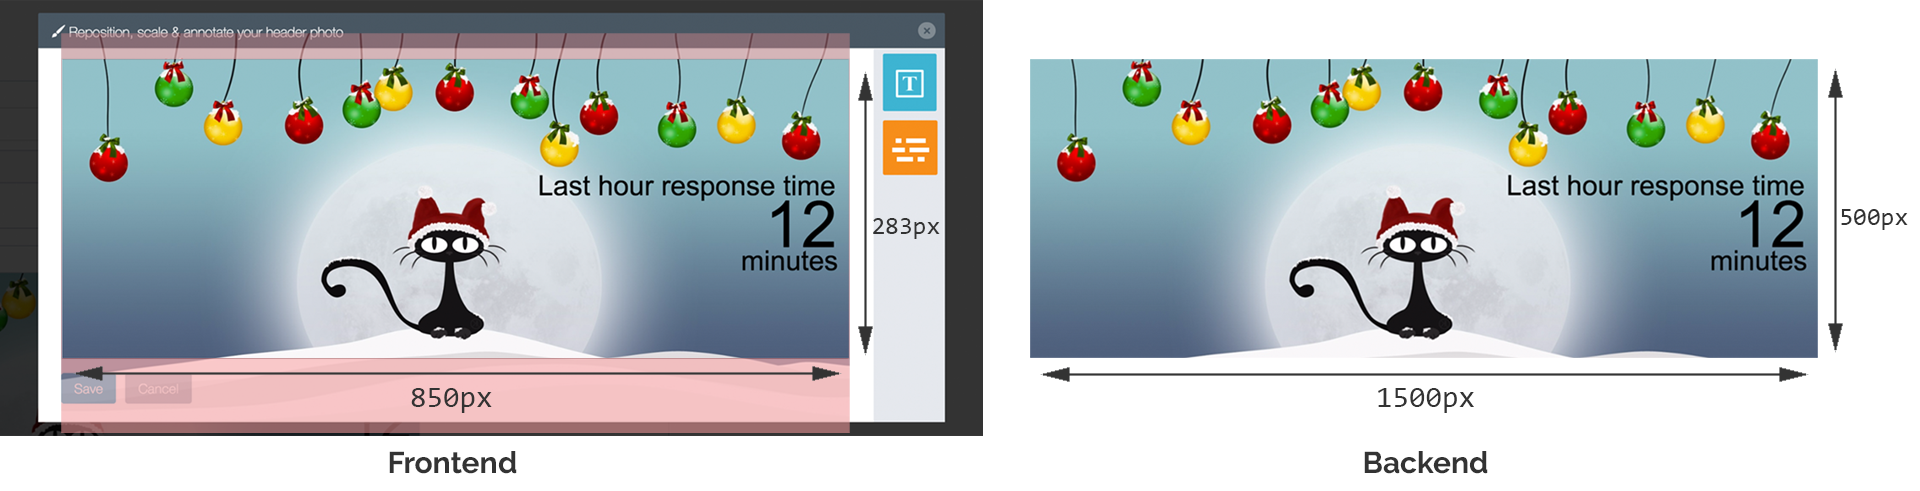
\includegraphics[width=1\textwidth]{Figuren/FrontToBack.png}
	\caption{Veranderingen in dimensies van Twitter omslagfoto}
	\label{fig:FrontToBackend}
\end{figure} 

Tijdens het verwerken van de annotaties zullen enkele functies asynchroon uitgevoerd worden. Om uiteindelijk een \textit{response} terug te kunnen sturen met de aangemaakte afbeelding, moet dus rekening gehouden worden met dit asynchrone gedrag. Daarom wordt gebruik gemaakt van een \texttt{Promise}. Wanneer het opstellen van het canvas succesvol verloopt, wordt deze \textit{promise} opgelost door de \texttt{resolve} functie. Wordt in de code gemerkt dat \'{e}\'{e}n of meerdere KPI's ontbreken, wordt de \texttt{reject} functie opgeroepen (zie codefragment \ref{lst:ResolvingStream}). 

Zoals vermeld in sectie \ref{BackendImplementationNodeJS} stelt Fabric.js enkele functies beschikbaar voor gebruik in een Node.js omgeving. Zo kan met behulp van de \texttt{loadFromJSON()} methode een canvas opgesteld worden vanuit JSON data. Wanneer het canvas opnieuw bestaat, worden alle objecten aangepast aan de nieuwe dimensies. De eerder berekende schalingsfactor (zie codefragment \ref{lst:NodeServicePromise}) wordt gebruikt om de positie, hoogte en breedte van ieder object op gepaste wijze te vergroten. Bij tekst objecten wordt de tekstgrootte hier ook mee vermenigvuldigd. Zo wordt exact dezelfde afbeelding bekomen zoals deze door de gebruiker aangemaakt werd maar met de correcte dimensies om te gebruiken op Facebook of Twitter. 

E\'{e}n van de belangrijkste \textit{features} van het annoteren is de mogelijkheid om KPI's te plaatsen op een afbeelding. Aangezien dit variabele waarden zijn, moeten ze ook om de zoveel tijd aangepast worden. Bij het aanspreken van de Node.js service worden naast de annotaties ook de pas berekende KPI's doorgegeven. Tijdens het schalen van de objecten wordt gekeken of het een object van het \texttt{textType} 'kpi' is. %maybe reference to that part?? \ref{AnnoterenVanAfbeelding}
Is dit het geval en is de corresponderende KPI aanwezig in de ontvangen data, kan de huidige tekst vervangen worden door de waarde van de KPI. 
 
\subsection{Exporteren van het canvas} \label{ExporterenVanHetCanvas}
Nu het canvas volledig is opgebouwd met de correcte afmetingen en KPI's, moet hieruit een afbeelding gegenereerd worden. Deze wordt dan uiteindelijk ingesteld als omslagfoto op Facebook of Twitter. Om de afbeelding te genereren wordt gebruik gemaakt van de \texttt{createPNGStream()} methode van Fabric. Bij het aanroepen van deze functie op het canvas wordt een \textit{stream} opgezet van omgezette data. %https://nodejs.org/api/stream.html
Op het moment dat deze stream data voortbrengt, wordt het \texttt{data} event uitgezonden. In de \textit{handler} van dit event kan dan verder gewerkt worden met de stukken data. Zo kan een nieuwe stream omgezet worden om een PNG bestand op te bouwen. % MSS VERWIJDEREN?? <--
Hoewel dit ook zijn toepassingen heeft, is dit in niet gewenst. De afbeeldingsdata moet namelijk teruggestuurd worden als \textit{response} zodat er verder mee gewerkt kan worden. 
%END EVENT -> ZET ALLE EVENTS TUSSEN AANHALINGSTEKENS!!!
Om te vermijden dat de foto eerst nog op de fileserver geplaatst moet worden, wordt er voor gekozen om onmiddellijk de base64 ge\"{e}ncodeerde afbeelding terug te sturen. Zoals in codefragment \ref{lst:Base64Generation} te zien is, worden de stukjes data aan een \textit{array} toegevoegd. Wanneer er geen data meer beschikbaar is wordt het \texttt{'end'} event uitgezonden. Bij het afhandelen van dit event zullen alle elementen van de \textit{array} geconcateneerd worden via de \texttt{Buffer.concat()} functie. Dit resulteert in een base64 ge\"{e}ncodeerde afbeelding die simpelweg als \textit{response} teruggestuurd kan worden. Er wordt gebruik gemaakt van een buffer omdat de \texttt{Buffer} klasse speciaal ontworpen is om rauwe binaire data te verwerken en dat is exact wat de PNG stream voorstelt. %https://nodejs.org/api/buffer.html#buffer_class_method_buffer_concat_list_totallength

%2 mogelijkheden: base64 doorsturen of op fileserver pushen en url doorsturen en dan terug afhalen. 
 %MSS IETS OVEr DE RESOLVE NOG ZEGGEN???!!!
\begin{lstlisting}[caption={renderer.js - aanmaken van base64},label=lst:Base64Generation,language=javascript]
var stream = fabricCanvas.createPNGStream();
var base64data = [];

stream.on('data', function (chunk) {
	base64data.push(chunk);
});

stream.on('end', function () {
	var result = Buffer.concat(base64data);
	console.log('Picture for ' + service + ' was successfully generated');
	resolve(result);
});
\end{lstlisting}

\subsection{Testen van de Node.js service}
Om correcte werking van de service te garanderen is het logisch dat hiervoor een test geschreven wordt. Hier moet dus de functionaliteit van een Node.js service getest worden. Om dit te verwezenlijken wordt gebruik gemaakt van Jest \ref{JestGettingStarted}. Dit \textit{framework} van Facebook maakt het zeer eenvoudig om JavaScript te testen. Jest wordt ge\"{i}nstalleerd via NPM zoals elke andere module. Voor de test uit te werken, worden enkele instellingen aangepast. Aangezien Jest zal gebruikt worden in een Node omgeving, wordt \textit{node} ingesteld als \texttt{testEnvironment} in het \texttt{package.json} bestand. 

Wat hier getest moet worden is het genereren van een afbeelding. Alle logica, die de annotaties en KPI's omzet in een afbeelding, zit reeds in een aparte module verwerkt (zie sectie \ref{OpbouwenCanvas}). In een nieuw test bestand, met een \texttt{.test.js} extensie, wordt de test opgezet. Deze test leest een reeds bestaande afbeelding in met behulp van de \texttt{fs} module waarna deze omgezet wordt naar base64. Daarna wordt een nieuwe afbeelding gegenereerd uit JSON data en KPI's. Uiteindelijk worden beide base64 \textit{strings} met elkaar vergeleken via de \texttt{expect()} methode en \texttt{toBe()} \textit{matcher}. Zijn beide ge\"{e}ncodeerde afbeeldingen aan elkaar gelijk, is de test geslaagd en werkt de code zoals het hoort. 

\begin{lstlisting}[caption={render.test.js - Testen van de service},label=lst:RenderTest,language=javascript]
test('test image rendering', () => {
	var image = fs.readFileSync('./test-twitter.png');
	var buffer = new Buffer(image).toString('base64');
	
	renderer.render(data, KPIs).then((data) => {
		expect(data.toString('base64')).toBe(buffer);
	}).catch((error) => {
		console.log(error);
	});
});
\end{lstlisting}

%MSS ERGENS UITLEGGEN WAT BASE64 IS??? IN VOORSTUDIE

%DOCKER & afbeeldingen compressie vlug vermelden! (3mb limit + fileserver storage size) + gebruike API calls (+ bv van Facebook, deleten van bestaande afbeeldingen etc!) en UniCrawler!!!

%Opzetten express server -> bodyparser voor json
%Aanmaken van 
%\subsection{Online plaatsen van Node.js server}
\subsection{Scheduling / Plannen van thema's}
Zoals vermeld in de beschrijving van het project (zie sectie \ref{BeschrijvingStageOpdracht}), kunnen gebruikers voor een bepaald profiel verschillende thema's inplannen. Om een thema te plannen kan gekozen worden tussen de reeds bestaande \textit{business hour schedules} of een aangepaste timing. 

\begin{figure}[H]
	\centering
	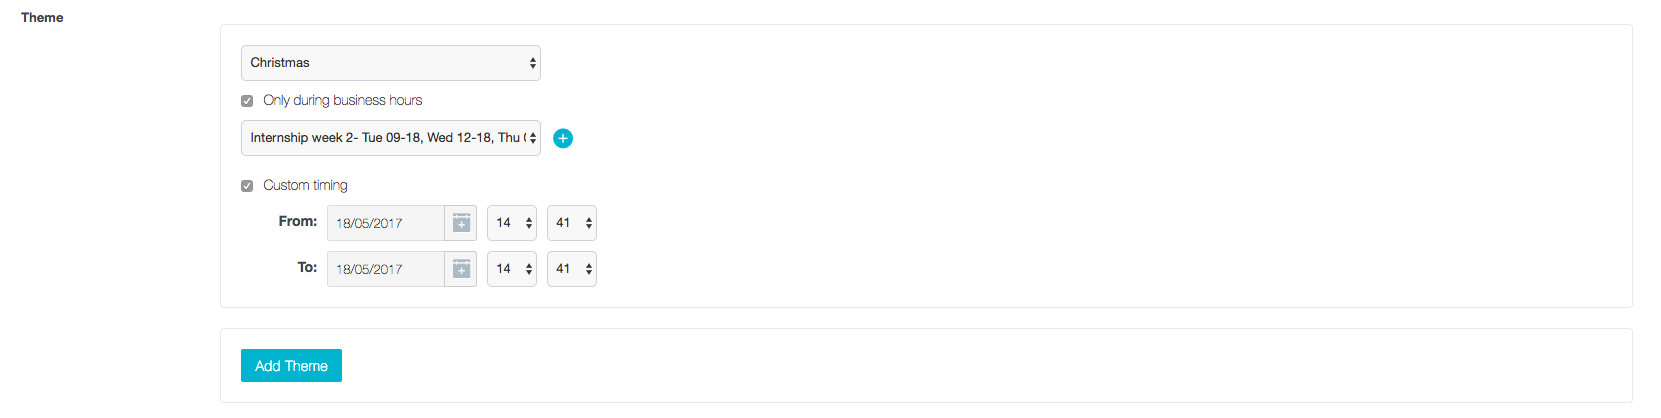
\includegraphics[width=1\textwidth]{Figuren/ThemeSet.png}
	\caption{Plannen van een thema}
	\label{fig:ThemeSet}
\end{figure}
%MSS TASK VERTALEN NAAR GWN TAAK??
Na het opstellen van een planning kan het profiel opgeslagen worden. Is dit een nieuw profiel, waar nog nooit iets voor werd ingesteld, dan wordt hiervoor een nieuwe \textit{task} aangemaakt. Een \textit{task} wordt gekenmerkt door een ID, een groep, een account, data, prioriteit, \texttt{nextScheduleDate} en \texttt{lastSuccessfulRun}. Aangezien \'{e}\'{e}n taak per profiel wordt aangemaakt, volstaat het om het profiel ID te gebruiken om de taken van elkaar te onderscheiden. De groep bepaald waartoe de taak behoort, hier dus de \texttt{profile-manager}. Als data wordt simpelweg het ID van het profiel gebruikt. De data bevat alles nodige informatie om de taak correct uit te voeren. Er wordt verwacht dat de \textit{task} onmiddellijk uitgevoerd wordt dus wordt als \texttt{nextScheduleDate} het huidige tijdstip genomen. 

Eens de taak aangemaakt is, wordt deze in de database opgeslagen en via de \textit{scheduler}, indien nodig, op de \textit{queue} geplaatst. Eens een taak in de \textit{queue} staat, wordt deze op zijn beurt uitgevoerd. Het uitvoeren van de taak gebeurt met behulp van de \textit{dispatcher}. Deze linkt de correcte \textit{handler} aan de taak zelf. In de \textit{handler} wordt de taak dan afgehandeld en wordt een volgende taak gepland. Het schema op Figuur \ref{fig:UniCrawler} toont het volledige proces. 

\begin{figure}[H]
	\centering
	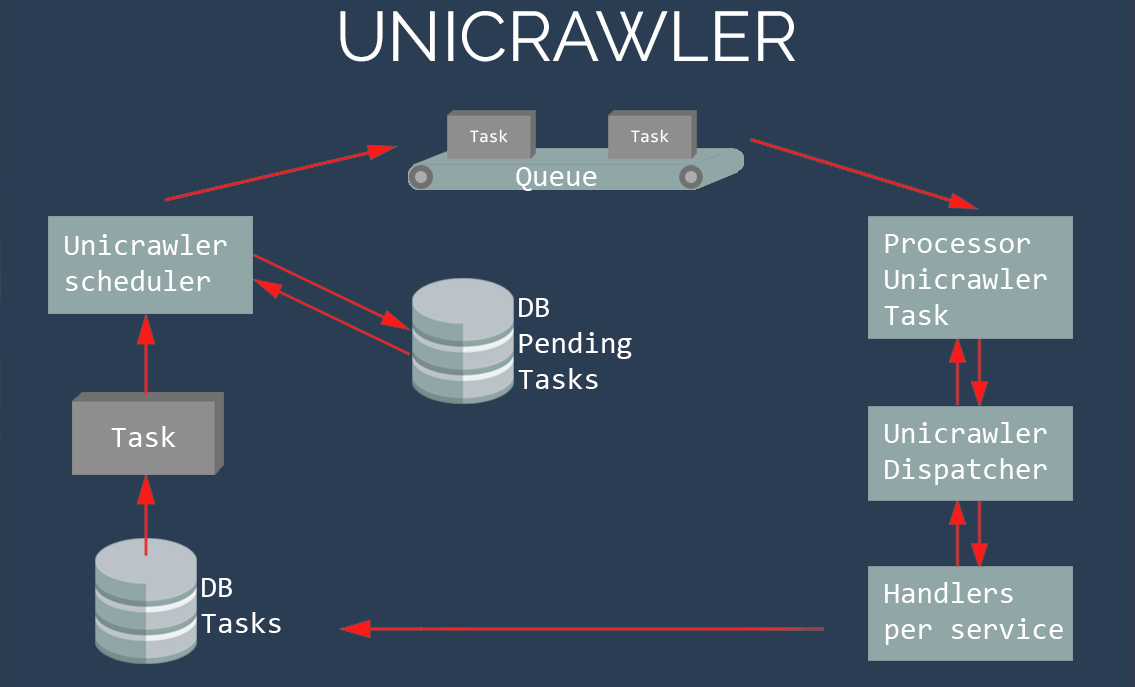
\includegraphics[width=1\textwidth]{Figuren/UniCrawler.png}
	\caption{UniCrawler}
	\label{fig:UniCrawler}
\end{figure}

Aangezien het de bedoeling is dat het thema op een profiel up-to-date gehouden wordt, wordt een taak om de vijf minuten herhaald. %REWRITE DIS SENTENCE <--
Bij het afhandelen van de taak worden verschillende checks uitgevoerd om te bepalen of het thema daadwerkelijk toegepast moet worden. Wanneer hetzelfde thema nog steeds actief is of de KPI's niet verandert zijn, is het nutteloos om de foto's opnieuw te genereren en te uploaden. Voor er overgegaan kan worden naar het toepassen van het thema, moet natuurlijk eerst bepaald worden welk thema actief moet zijn. 

Om dit te weten te komen, wordt gebruik gemaakt van een algoritme. Dit algoritme haalt voor een profiel alle ingeplande thema's op. Voor ieder thema wordt gekeken of deze een aangepaste \textit{timing} bevat of \textit{business hours} of beide. Valt het huidige tijdstip (waarop de taak dus wordt afgehandeld) binnen de ingestelde \textit{timing} dan wordt alle informatie over dat bepaalde thema bijgehouden. Hier moet vermeld worden dat tijdstippen uitgedrukt worden in Unix tijd om het vergelijken te vereenvoudigen. Eens de \textit{custom timing} bekeken is, worden alle ingestelde \textit{business hours schedules} overlopen. Gebruikers kunnen namelijk meerdere \textit{schedules} selecteren om zo de planning gedetailleerder te maken. De tijdstippen van deze \textit{schedules} worden vergeleken met het reeds berekende tijdstip en het meest recente wordt toegevoegd aan een lijst. Uit deze lijst wordt dan het meest recentste tijdstip genomen. Zo wordt het thema gevonden dat op dat moment actief moet zijn op basis van de \textit{business hours schedules}. Uiteindelijk wordt de berekende \textit{custom timing} vergeleken met de \textit{business hours} om te bepalen wat de bovenhand neemt. 

Wordt dit algoritme op iedere set (zie Figuur \ref{fig:ThemeSet}) toegepast, wordt uiteindelijk een lijst bekomen met het tijdstip van iedere set die op dat moment actief kan zijn. Met behulp van een sorteermethode worden alle sets aflopend geordend. De eerste in de lijst (met de hoogste waarde) is dan het actieve thema en moet dus ingesteld worden op het profiel. Wordt noch een \textit{custom timing} noch een \textit{business hours schedule} gevonden, dan wordt deze set eenvoudigweg aan dezelfde lijst toegevoegd met een timestamp die gelijk is aan 0. Het thema in deze set zal dus enkel actief zijn wanneer geen andere sets die aan de eisen voldoen, aanwezig zijn. Sets zonder enige specificaties kunnen dus als standaard thema voor een profiel ingesteld worden. 

%MAYBE DELETE?
Verschillende sets kunnen dus zo geconfigureerd worden dat een complexe planning van thema's ontstaat. Zo kunnen gebruikers bijvoorbeeld een standaard thema ingesteld hebben voor hun profiel maar wordt tijdens de openingsuren op de omslagfoto aangegeven dat het bedrijf open is. Op bepaalde feestdagen zoals Kerstmis of Pasen kan dan weer een aangepaste profielfoto getoond worden. 

\subsection{Uploaden naar sociale media}
Elke vijf minuten bestaat de kans dat een thema toegepast wordt en dus ook foto's ge\"{u}pload moeten worden naar Facebook of Twitter. Binnen CX Social wordt reeds gebruik gemaakt van de Application Programming Interface (API) van deze platformen waardoor er reeds code aanwezig is voor het maken van een \textit{request} naar elk van deze services. Deze code zal ook een correct authenticatie token, voor de ingelogde gebruiker, met de \textit{request} meegeven. %MSS WEGLATEN <-- ? MEER UITLEG EROVER!! OAUTH 2 ENZO!!
Er moet dus enkel een \textit{request} gestuurd worden naar de specifieke \textit{endpoints} waarmee profielfoto, omslagfoto en profielinformatie aangepast worden. 

\textbf{Twitter} \break
Om de omslagfoto van een Twitter-profiel aan te passen wordt gebruik gemaakt van de \texttt{/account/update{\_}profile{\_}banner} \textit{endpoint} \cite{TwitterAPIDoc}. De afbeelding zelf kan base64 ge\"{e}ncodeerd of als \textit{raw image data} meegegeven worden. Aangezien de omslagfoto's telkens door de Node.js service worden gegenereerd en dus in het base64 formaat ontvangen worden (zie sectie \ref{ExporterenVanHetCanvas}), kand de afbeelding rechtstreeks meegegeven worden aan het \textit{endpoint}. Zoals te zien in codefragment \ref{lst:TwitterAPICall} worden de URL naar de \textit{endpoint}, de afbeelding, \textit{request} methode en enkele opties verwacht om de \textit{call} te maken. Een van de opties is het verwachte antwoord op de \textit{request}. Dit kunnen zowel een HTTP status codes 200 (OK), 201 (Created) of 202 (Accepted) zijn. 

\begin{lstlisting}[caption={Uploaden van omslagfoto naar Twitter},label=lst:TwitterAPICall,language=PHP]
try {
	$updateBanner = $this->call(
		self::API_VERSION . '/account/update_profile_banner',
		array(
			'banner' => $image
		),
		'POST',
    	/* $multipart = */ false,
		/* $options = */ array(
		'expectedResponseCodes' => array(200, 201, 202)
	)
);

} catch (Exception $ex) {
	throw $ex;
}
\end{lstlisting}

Het uploaden van de profielfoto verloopt op gelijkaardige manier. Via de \texttt{/account/updateo{\_}profileo{\_}image} \textit{endpoint} wordt de base64 ge\"{e}ncodeerde afbeelding naar Twitter gestuurd \cite{TwitterAPIDoc}. In tegenstelling tot de omslagfoto moet een profielfoto niet geannoteerd worden. Hierdoor kan de afbeelding simpelweg vanop de fileserver gehaald worden. Deze foto wordt dan base64 ge\"{e}ncodeerd voor gebruik op Twitter.

\textbf{Facebook} \break
De Graph API van Facebook biedt de mogelijkheid om omslag-en profielfoto aan te passen. Dit is echter een heel stuk complexer bij Facebook dan bij Twitter. %MSS REMOVE? <--
Facebook verwacht namelijk dat gebruikers een foto, die reeds op hun tijdlijn staat, zullen instellen als omslagfoto. Dit betekent dat een foto eerst ge\"{u}pload wordt naar Facebook waarna deze als omslagfoto of profielfoto wordt ingesteld. Dit zorgt ervoor dat de foto niet enkel in het album met tijdlijnfoto's maar ook in het album met omslagfoto's of profielfoto's terecht komt. Wordt aangenomen dat een foto om de vijf minuten ge\"{u}pload wordt, is al snel duidelijk dat de verschillende albums rond de 300 foto's zullen bevatten na \'{e}\'{e}n dag. 

Dit is natuurlijk niet de bedoeling dus wordt dit probleem op volgende manier opgelost. %ISDA JUIST??? <--

Met behulp van de \texttt{/page-id/photos} \textit{edge} wordt een foto naar Facebook ge\"{u}pload. Een foto naar een pagina uploaden kan op twee manieren: via een verwijzing naar een foto die reeds op het internet staat (dus via een URL) of de afbeelding toevoegen als \texttt{multipart/form-data}. Mits de gegenereerde foto's nog niet beschikbaar zijn op het internet, wordt voor de laatste methode geopteerd. Naast een \textit{access token} en wat opties, wordt het pad naar het bestand als \textit{source} parameter meegegeven. Aangezien het niet gewenst is om een notificatie te krijgen wanneer een omslag-of profielfoto wordt gewijzigd, wordt de \textit{no{\_}story} parameter ook actief gezet (zie codefragment \ref{lst:FacebookAPICallUpload}) \cite{FacebookPagePhotos}. 

\begin{lstlisting}[caption={Uploaden van een foto naar Facebook},label=lst:FacebookAPICallUpload,language=PHP]
$uploadedPhotoId = $this->call(
	'/' . Services_Facebook_Migrations::VERSION_2_8 . '/' . $this->getServiceId() . '/photos',
	$this->getAccessToken(),
	Services_Facebook_Manager::MODE_JSON,
	'POST',
	array(
		'source' => '@' . realpath($tempFile),
		'no_story' => true,
	),
	/* options */ array( 
		'postFieldsAsString' => false,
		'timeout' => static::UPLOAD_TIMEOUT,
	)
);
\end{lstlisting}

%ASK WHERE THE AUTH TOKEN COMES FROM! https://developers.facebook.com/tools/explorer?method=GET&path=me%2Faccounts&version=v2.9
%https://en.wikipedia.org/wiki/OAuth  https://www.youtube.com/watch?v=L1PDqJkedZ0

%Facebook -> Dit is zeker niet de beste oplossing maar momenteel de meest gebruiksvriendelijke. 
Na het uploaden van een foto naar de tijdlijn wordt als antwoord het ID van deze foto ontvangen. Met een call naar de pagina zelf kan deze foto ingesteld worden als omslagfoto. Parameters hierbij zijn \textit{cover} (het ID van de foto) en \textit{offset{\_}x} en \textit{offset{\_}y} van de omslagfoto (zie codefragment \ref{lst:FacebookAPICallCover}). Ook hier wordt de \textit{no{\_}feed{\_}story} parameter toegevoegd om te vermijden dat volgers van de pagina, om de x aantal minuten, een notificatie ontvangen. 

Uiteindelijk worden enkele maatregelen getroffen om het aantal foto's in de albums te beperken. Zo wordt v\'{o}\'{o}r het uploaden van een nieuwe foto, het ID van de huidige afbeelding opgehaald. Na het instellen van de nieuwe afbeelding, kan de andere foto via het ID uit het album verwijdert worden. Uiteindelijk wordt de foto ook uit het tijdlijn album verwijdert. Op deze manier wordt het aantal foto's in de albums tot een minimum beperkt.

\begin{lstlisting}[caption={Instellen van omslagfoto op Facebook},label=lst:FacebookAPICallCover,language=PHP]
$coverPhoto = $this->call(
	'/' . Services_Facebook_Migrations::VERSION_2_8 . '/' . $this->getServiceId(),
	$this->getAccessToken(),
	Services_Facebook_Manager::MODE_JSON,
	'POST',
	array(
		'cover' => $uploadedPhotoId['id'],
		'offset_x' => 0,
		'offset_y' => 0,
		'no_feed_story' => true
	),
	array(
		'timeout' => static::UPLOAD_TIMEOUT,
	)
);
\end{lstlisting}

Het uploaden van een profielfoto verloopt op gelijkaardige manier. Het instellen als avatar gebeurt hier via de \texttt{/page-id/picture} edge van de Graph API \cite{FacebookPagePicture}. Als parameters worden \textit{photo} (het ID van de foto in het tijdlijn album), \textit{width}, \textit{height} en \textit{no{\_}feed{\_}story} meegegeven. De hoogte en breedte van de foto worden ingesteld op 200 pixels omdat Facebook een foto van minimum 180 op 180 pixels verwacht \cite{FacebookDimensions}. 

Net zoals bij het instellen van een omslagfoto moeten de vorige profielfoto en de ge\"{u}ploade foto verwijdert worden om een overvloed aan foto's te vermijden. In tegenstelling tot de omslagfoto, kan het ID van de huidige profielfoto niet opgehaald worden. Wanneer het ID niet beschikbaar is, kan ook de correcte foto niet verwijdert worden. Om dit probleem op te lossen wordt het volledige album van profielfoto's opgehaald. Aangezien de eerste foto in dit album de huidige profielfoto is, kan het ID hier uit gehaald worden om zo de foto te verwijderen. Hoewel deze methode het ene probleem oplost, veroorzaakt het een ander. Het verwijderen van de eerste foto in het album zorgt er voor dat gebruikers zelf geen profielfoto kunnen instellen via Facebook zelf. Deze zal namelijk verwijdert worden wanneer een thema wordt toegepast. De kans dat dit voorkomt is echter miniem omdat verwacht wordt van gebruikers dat ze de foto aanpassen vanuit de Profile Manager en niet op het profiel zelf. 

\iffalse
\subsection{Afbeeldingcompressie?}
Bij het uitwerken van dit project werd ook even stilgestaan bij afbeeldingcompressie. Het is namelijk niet gewenst om zeer grote afbeeldingen in te laden en/of op te slaan. Gelukkig kunnen heel wat problemen vermeden worden bij dit project. Een foto moet slechts op \'{e}\'{e}n plaats daadwerkelijk opgeslagen worden. Wanneer de gebruiker een nieuw thema aanmaakt, kunnen een omslagfoto en avatar gekozen worden. Bij het selecteren van de foto wordt deze naar de fileserver ge\"{u}pload. Ook hier wordt geen compressie toegepast maar er wordt gezorgd dat de bestanden niet groter zijn dan 3 megabyte. 

Waar op andere plaatsen in het project gebruik gemaakt wordt van foto's, wordt telkens met de base64 ge\"{e}ncodeerde foto gewerkt. Dit betekent dat de foto simpelweg als tekst verstuurd kan worden. Deze foto's worden opgebouwd met onder andere het bestand dat reeds op de fileserver staat. 
\fi


 %telkens de link naar het ge\"{u}ploade bestand gebruikt. 
